\RequirePackage{luatex85}
\documentclass[leqno]{ltjsarticle}
\usepackage{luatexja-fontspec}
\usepackage[top=10truemm,bottom=10truemm,left=20truemm,right=20truemm]{geometry}
\usepackage{luatexja} 
\usepackage{multicol,amsmath,amssymb,mathtools,ascmac,amsthm,amscd,physics,comment,dcolumn,titlesec,mathrsfs,test,tikz-cd}
\usetikzlibrary{arrows.meta,calc}
\titleformat*{\section}{\Large\bfseries}
\setlength{\parindent}{0pt}
\pagestyle{empty}
%\everymath{\displaystyle}
\begin{document}
%{\textbf{\Large{}}}\hspace{\fill} {\texttt{\Large{04A21051}}}{\Large{Yudai Yamamoto}}\\
\section{三角圏の公理}
	加法圏$\D$と自己同値$[1]$に対して以下を満たすとき三角圏と呼ぶ.
	\begin{itemize}
		\item[(i)]
			\[E\xrightarrow{\id}E\rightarrow 0 \rightarrow E[1]\]
			は完全三角形.
		\item[(ii)]
			\[
		\begin{tikzcd}
			E_1\ar[r]\ar[d,"f"]& E_2\ar[r]\ar[d,"g"]& E_3\ar[r]\ar[d,"h"] & E_1[1]\ar[d,"f\texttt{[1]}"]\\
			F_1\ar[r]& F_2\ar[r]& F_3\ar[r] & F_1[1]\\
		\end{tikzcd}
			\]
			上の可換図式において,$f,g,h$が同型で$F_1\rightarrow F_2\rightarrow F_3 \rightarrow F_1[1]$が完全三角形なら$F_1\rightarrow F_2\rightarrow F_3 \rightarrow F_1[1]$も完全三角形
		\item[(iii)]
			任意の$E\xrightarrow{f}F$は
			\[E\xrightarrow{f} F\rightarrow G \rightarrow E[1]\]
		と完全三角形に拡張できる.
	\item[(iv)]
		\[
			E_1\xrightarrow{u} E_2\xrightarrow{v} E_3\xrightarrow{w}  E_1[1]
	\]
	が完全三角形であることと
	\[
		E_2\xrightarrow{v} E_3\xrightarrow{w} E_1\xrightarrow{-u[1]}  E_2[1]
	\]
	が完全三角形であることが同値.
	\item[(v)]
		\[
		\begin{tikzcd}
			E_1\ar[r]\ar[d,"f"]& E_2\ar[r]\ar[d,"g"]& E_3\ar[r]\ar[d,"h",dotted] & E_1[1]\ar[d,"f\texttt{[1]}"]\\
			F_1\ar[r]& F_2\ar[r]& F_3\ar[r] & F_1[1]\\
		\end{tikzcd}
	\]
	2つの完全三角形と図式を可換にする$f,g$が存在したとき,すべての四角形を可換にする$h$が存在する.

	\item[(vi)]
		八面体公理\\
			\[
				\begin{tikzcd}[row sep=5pt]
			E \ar[r,"f"]& F\ar[r,"h"]& Z \ar[r]& E[1]\\
			E \ar[r,"g\circ f"]& G\ar[r,"l"]& Y \ar[r]& E[1]\\
			F \ar[r,"g"]& G\ar[r,"k"]& X \ar[r]& F[1]\\
		\end{tikzcd}
			\]
	上記の3つの完全三角形に対して,以下の図式のすべての四角形を可換にし,4行目を完全三角形にするような$u,v,w$が存在する.
			\[
		\begin{tikzcd}
			E \ar[r,"f"]\ar[d,equal]& F\ar[r,"h"]\ar[d,"g",swap]& Z\ar[d,"u",dotted] \ar[r]& E[1]\ar[d,equal]\\
			E \ar[r,"g\circ f"]\ar[d,"f",swap]& G\ar[r,"l"]\ar[d,equal]& Y\ar[d,"v",dotted] \ar[r]& E[1]\ar[d,"f\texttt{[1]}"]\\
			F \ar[r,"g"]\ar[d,"h",swap]& G\ar[r,"k"]\ar[d,"l",swap]& X \ar[r]\ar[d,equal]& F[1]\ar[d,"h\texttt{[1]}"]\\
			Z \ar[r,"u",dotted]& Y\ar[r,"v",dotted]& X \ar[r,"w",dotted]& Z[1]\\
		\end{tikzcd}
			\]
	\end{itemize}
\section{t-structure}
	\mydef{
		$\D$を三角圏.充満部分三角圏$\D^{\le 0},\D^{\ge 0}\subset\D$が次の条件を満たすとき,$(\D^{\le 0},\D^{\ge 0})$を$\D$のt-構造と呼ぶ.
		$\D^{\le n}\coloneq\D^{\le 0}[n],\hspace{3mm}\D^{\ge n}\coloneq\D^{\ge 0}[n] $
		\begin{itemize}
			\item[(i)]
				$\D^{\le 0}\subset\D^{\le 1}\hspace{3mm}\D^{\ge 1}\subset\D^{\ge 0} $
			\item[(ii)]
				$\D^{\ge 1}\subset (\D^{\le 0})^\perp$\\
				つまり,$\forall E\in \D^{\le 0},\ \forall F\in\D^{\ge 1},\ \Hom_{\D}(E,F)=0$
			\item[(iii)]
				任意の$E\in\D$に対して
				\[\tau_{\le 0}E\rightarrow E \rightarrow \tau_{\ge 1}E\rightarrow \tau_{\le 0}E[1]\]
				となるような$\tau_{\le 0}E\in\D,\ \tau_{\ge 1}E\in\D^{\ge 1}$が存在する.
		\end{itemize}
	}

	\myprop{
		\begin{itemize}
				\item[(i)]$\D^{\ge 1}=(\D^{\le 0})^{\perp}$
				\item[(ii)]$E$に対して,$\tau_{\le 0}E, \tau_{\ge 1}E$は同型を除いて一意に定まる.
		\end{itemize}
	}
	\begin{proof}
		$E\in\mathcal (\D^{\le 0})^\perp$ を任意にとる.定義より以下の完全三角形がとれる.
				\[\tau_{\le 0}E\rightarrow E \rightarrow \tau_{\ge 1}E\rightarrow \tau_{\le 0}E[1]\]
		定義より,$\tau_{\le 0}E\rightarrow E$は0射であるので,$\tau_{\ge 1}E\simeq$ 
				
	\end{proof}


	射影的代数曲線$\defi$射影空間$\PP^n$内の1次元部分多様体\\ \\
\section{安定性条件}
	

	\mydef{
		Abel圏$\A$上の安定性条件とは群準同型
		\[Z\colon K(\A)\to \CC\]
		で以下を満たすもの
\begin{itemize}
	\item[(i)]
		$\forall E(\neq 0)\in\A, Z(E)\in\HH\coloneq \{re^{i\pi\phi}\mid r>0, 0<\phi \le 1\}$
	\item[(ii)]
		任意の$E\in\A$に対してHNフィルトレーションが存在する.
		\[0=E_0\subset E_1\subset \cdots \subset E_k = E\]
		で各$F_i = E_i/E_{i-1}$が$Z$について$Z$-半安定.
\end{itemize}
$E(\neq 0)$が$Z$-半安定とは任意の部分対象$0\neq F\subsetneq E$に対して,$\arg Z(F) \le \arg Z(E)$
ここで,
\[\phi(E)\coloneq \frac{1}{\pi}\arg Z(E) \]
と定める.
	}
\mylem{
	$E,F\in\D$が半安定で$\phi(E)>\phi(F)$とき,
	\[\Hom_{\D}(E,F)=0\]
}
\begin{proof}
	$f\in\Hom_{\D}(E,F)$が$0$でないと仮定する.
	\[0\rightarrow\Ker f\rightarrow E \rightarrow \Im f \rightarrow 0\]
	の完全列が存在して$E$が半安定対象であることから$\phi(\Im f)\ge\phi(E)$.$\Im f\neq 0$が$F$の部分対象で$F$も半安定であることから$\phi(F)\ge\phi(\Im f)$.これらを合わせると$\phi(F)\ge\phi(E)$.仮定に矛盾.
\end{proof}

\mylem{
	$\A\colon$アーベル圏,群準同型$Z\colon K(\A)\to \CC$が次の条件を満たすとき,HNフィルトレーションが存在する.つまり$Z$が安定性条件を定める.
	\begin{itemize}
		\item[(i)]
		全射の無限列
	\[E_1\twoheadrightarrow E_2\twoheadrightarrow E_3\twoheadrightarrow\cdots  \]
	で$\phi (E_i)> \phi (E_{i+1})$となるものは存在しない.
\item[(ii)]
		無限降下列
	\[E_1\supset E_2\supset E_3\supset \cdots  \]
	で$\phi (E_{i+1}) > \phi(E_i)$となるものは存在しない.
\end{itemize}
}
\begin{proof}\hfill\\
	\begin{screen}
	Step 1\hspace{5mm}\\
	\bullet 任意の対象$E\in\A$には$\phi(A) \ge \phi(E)$を満たす半安定な部分対象$A$が存在する.\\
	\bullet 任意の対象$E\in\A$には$\phi(E) \ge \phi(B)$を満たす半安定な対象$B$と全射$E\twoheadrightarrow B$が存在する.
\end{screen}
	$E$が半安定ならOK.そうでないなら$\phi(E')>\phi(E)$となる部分対象$E'(\subsetneq E)$がとれる.\\
	これが無限回繰り返されると条件の(ii)に矛盾するので有限回でとまる.この極小となる$A$をとれば半安定である.\\
	同様に$E$が半安定なら全射$E\xrightarrow{\id}E$がとれてOK.そうでないとき,$E'(\subsetneq E)$で,$\phi(E')>\phi(E)$が存在して,$B'\coloneq E/E'$と定めると$\phi(E)\ge\phi(B')$であり,$E\twoheadrightarrow E/E'$がとれて,有限回でこの操作はとまるのでいずれ半安定になる.
\begin{center}
	\usetikzlibrary{arrows.meta}

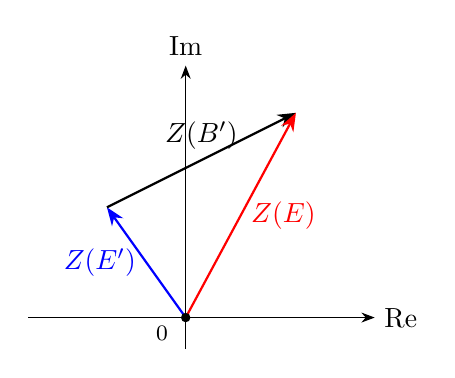
\begin{tikzpicture}[scale=2, >=Stealth]

  % 原点を中心に設定
  \coordinate (O) at (0,0);

  % 各ベクトルの終点
  \coordinate (E') at (-0.5,0.7);     % Z(A)
  \coordinate (B') at (1.2,0.6);    % Z(E/A)
  \coordinate (E) at ($(E')+(B')$); % Z(E) = Z(A) + Z(E/A)

  % 軸
  \draw[->] (-1,0) -- (1.2,0) node[right] {\(\Re\)};
  \draw[->] (0,-0.2) -- (0,1.6) node[above] {\(\Im\)};

  % Z(A) ベクトル(青)
  \draw[->, thick,blue] (O) -- (E') node[midway, left] {\(Z(E')\)};

  % Z(E/A) ベクトル(緑):Aの先から
  \draw[->, thick] (E') -- (E) node[midway,above] {\(Z(B')\)};

  % Z(E) ベクトル(赤):原点から
  \draw[->, thick,red] (O) -- (E) node[midway, right] {\(Z(E)\)};

  % 原点
  \fill (O) circle (0.03);
  \node at (-0.15, -0.1) {\footnotesize 0};

\end{tikzpicture}
\end{center}

	\begin{screen}
		Step 2\\
			$E\twoheadrightarrow B$が次の条件をみたすときmdqと呼ぶ.\\
			\bullet $\phi(E)\ge\phi(B)$\\
			\bullet 任意の$E\twoheadrightarrow B'$に対して,$\phi(B')\ge \phi(B)$であり,$\phi(B')=\phi(B)$なら
			\[E\twoheadrightarrow B\twoheadrightarrow B'\]
			と分解.\\
			任意の対象$E$はmdqを持つ.
	\end{screen}
	$E\twoheadrightarrow B'$において$B'$が半安定でないならStep 1から半安定な対象$B''$で$\phi(B')>\phi(B'')$と$B'\twoheadrightarrow B''$がとれるので,$B'$が半安定なときについて示せばよい.同様にmdqの$B$は半安定でなければならない.\\
$E$が半安定対象のとき,任意の全射$E\twoheadrightarrow B'$に対して,短完全列
\[0\rightarrow \Ker f\rightarrow E\xrightarrow{f} B'\rightarrow 0\]
が存在するので$Z(B') = Z(E) - Z(\Ker f)$.安定対象なので,$\phi(\Ker f)\le \phi(E)$
\begin{center}
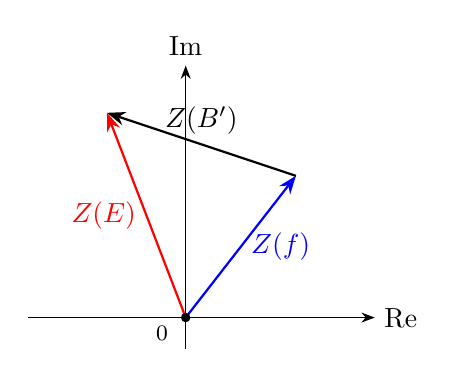
\begin{tikzpicture}[scale=2, >=Stealth]

  % 原点を中心に設定
  \coordinate (O) at (0,0);

  % 各ベクトルの終点
  \coordinate (Ker) at (0.7,0.9);     % Z(A)
  \coordinate (B') at (-1.2,0.4);    % Z(E/A)
  \coordinate (E) at ($(Ker)+(B')$); % Z(E) = Z(A) + Z(E/A)

  % 軸
  \draw[->] (-1,0) -- (1.2,0) node[right] {\(\Re\)};
  \draw[->] (0,-0.2) -- (0,1.6) node[above] {\(\Im\)};

  % Z(A) ベクトル(青)
  \draw[->, thick,blue] (O) -- (Ker) node[midway, right] {\(Z(\Ker f)\)};

  % Z(E/A) ベクトル(緑):Aの先から
  \draw[->, thick] (Ker) -- (E) node[midway,above] {\(Z(B')\)};

  % Z(E) ベクトル(赤):原点から
  \draw[->, thick,red] (O) -- (E) node[midway, left] {\(Z(E)\)};

  % 原点
  \fill (O) circle (0.03);
  \node at (-0.15, -0.1) {\footnotesize 0};

\end{tikzpicture}
\end{center}
したがって,$\phi(B')\ge\phi(E)$となり$E$が半安定対象のとき,$E\xrightarrow{\id}E$はmdqとなる.\\
そうでないとき,step1より$\phi(A)>\phi(E)$なる半安定対象$A\subsetneq E$と
\[0\rightarrow A\rightarrow E\rightarrow E'\rightarrow 0\]
という完全列が存在する.$\phi(A)>\phi(E)>\phi(E')$となっている.$E'\twoheadrightarrow B$が$E'$のmdqとなっているとき,合成$E\twoheadrightarrow B$は$E$のmdqであることを示す.\\
\because $E\twoheadrightarrow B'$を半安定で$\phi(B')\le \phi(B)$となっているとすると
\[\phi(A)>\phi(E)>\phi(E')\ge\phi(B)\ge\phi(B')\]
$A,B'$は半安定対象であり,前の補題より$\Hom_{\D}(A,B')=0$
\[\begin{tikzcd}
	A \ar[r,hookrightarrow]\ar[rd,"0",swap,]& E\ar[r,twoheadrightarrow]\ar[d,twoheadrightarrow]& E/A = E'\ar[ld,dotted]\\
								 &B'
\end{tikzcd}\]
図式のように可換にする全射が普遍性から存在する.$E'\twoheadrightarrow B$がmdqなので$\mu(B')=\mu(B)$となり,mdqの条件より$E'\twoheadrightarrow B\twoheadrightarrow B'$と経由する.したがって$E\twoheadrightarrow B\twoheadrightarrow B'$が存在し,$E\twoheadrightarrow B$がmdqであることがわかる.\\
$E'$がmdqでない場合は$E$を$E'$に取り替えて議論を繰り返すことと条件(ii)から有限回でとまるのでmdqの存在がわかる.

	\begin{screen}
		Step 3\\
		任意の$E\in\A$はHNフィルトレーションをもつ.
	\end{screen}
	$0$でない$E\in\A$を任意にとる.$E$が半安定なら$0\subset E$がHNフィルトレーションを与えている.そうでないとき,$E\twoheadrightarrow B^1$をmdqとして
	\[0\rightarrow E^1 \rightarrow E\rightarrow B^1\rightarrow 0\]
	をとる.$E^1$が半安定であるなら$0\subsetneq E^1\subsetneq E$がHNフィルトレーションになっている.($E/E^1\simeq B$でmdqの$B$が半安定であるため).$E^1$がmdqでないとき,$E^1\twoheadrightarrow B^2$をmdqとして
	\[0\rightarrow E^2\rightarrow E^1\rightarrow B^2\rightarrow 0\]
	$Q=E/E^2$とすると,$E\twoheadrightarrow B^1$がmdqであることから$\phi(Q)\ge\phi(B^1)$であり,次の短完全列
	\[0\rightarrow B^2\rightarrow Q\rightarrow B^1\rightarrow 0\]
	\begin{center}
	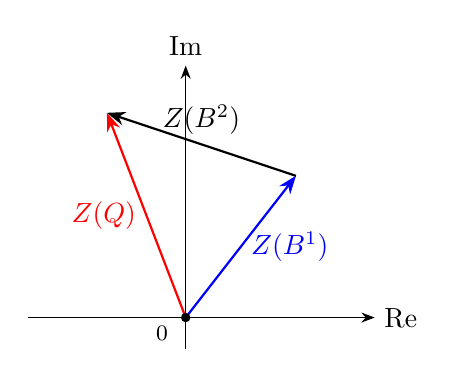
\begin{tikzpicture}[scale=2, >=Stealth]

		% 原点を中心に設定
		\coordinate (O) at (0,0);

		% 各ベクトルの終点
		\coordinate (B1) at (0.7,0.9);     % Z(A)
		\coordinate (B2) at (-1.2,0.4);    % Z(E/A)
		\coordinate (Q) at ($(B1)+(B2)$); % Z(E) = Z(A) + Z(E/A)

		% 軸
		\draw[->] (-1,0) -- (1.2,0) node[right] {\(\Re\)};
		\draw[->] (0,-0.2) -- (0,1.6) node[above] {\(\Im\)};

		\draw[->, thick,blue] (O) -- (B1) node[midway, right] {\(Z(B^1)\)};

		\draw[->, thick] (B1) -- (Q) node[midway,above] {\(Z(B^2)\)};

		\draw[->, thick,red] (O) -- (Q) node[midway, left] {\(Z(Q)\)};

		% 原点
		\fill (O) circle (0.03);
		\node at (-0.15, -0.1) {\footnotesize 0};

	\end{tikzpicture}
\end{center}
から$\phi(B^2)\ge\phi(Q)$が得られる.$\phi(B^2)=\phi(Q)=\phi(B^1)$と仮定すると,$E\twoheadrightarrow B^1$がmdqであることから$E\twoheadrightarrow B^1\twoheadrightarrow Q$となって,$B^1$と$Q$の双方向に全射があることから$B^1\simeq Q$となり,$B^2=0$.これは矛盾.したがって,$\phi(B^2)>\phi(B^1)$が成り立つ.この操作は条件(ii)より有限回でとまり,その商は半安定なのでHNフィルトレーションを得る.
\end{proof}

\mydef{
	$\D\colon$三角圏.$\D$上の安定性条件とは,$\D$の有界な$t$-構造のHeart $\A\subset\D$と$\A$と$\A$上の安定性条件
	\[Z\colon K(\D)=K(\A)\to\CC\]
	$(Z,\A)$のことである.
}

	三角圏$\D$におけるスライスとは部分圏の族$\{\P(\phi)\}_{\phi\in\RR}\subset\D$で次の条件を満たすもの\\
	\bullet $\forall\phi\in\RR, \P(\phi + 1) = \P(\phi)[1]$\\
	\bullet $\phi_1>\phi_2$で$E_i\in\P(\phi_i)$ならば$\Hom_{\D}(E_1,E_2)=0$\\
	\bullet 任意の対象$E\in\D$に対して,
	\[
		\begin{tikzcd}
			0\ar[r,equal]& E_0\ar[rr]& & E_{1}\ar[r]\ar[ld] &\cdots\ar[r] &E_{n-2}\ar[rr]&&E_{n-1}\ar[ld]\ar[rr]&&E\ar[ld]\\
									 &&F_{1}\ar[lu,dotted,"{[1]}"] &&&&F_{n-1}\ar[lu,dotted,"{[1]}"]&&F_n\ar[lu,dotted,"{[1]}"]
		\end{tikzcd}
	\]
	$F_i\in\P(\phi_i)$

	\mylem{
		$\D$上に安定性条件をあたえることと,$\D$上のスライス$\P$と群準同型$Z\colon K(\D)\to\CC$の組$(Z,\P)$で,任意の$\phi\in\RR$と$0\neq E\in\P(\phi)$に対して$Z(E)\in\RR_{>0}e^{i\pi\phi}$を与えることは同値.
	}
	\begin{proof}
		安定性条件$(Z,\A)\rightarrow$スライス$\P$の構成\\
		各$0<\phi\le 1$に対して,
		\[\P(\phi)\coloneq \{E\in\A\mid E\colon Z\text{-半安定 }Z(E)\in\RR_{>0}e^{i\pi\phi}\}\cup \{0\}\]
		$\phi\in\RR,\phi\in(k,k+1]$となる整数$k$をとって
		\[\P(\phi)\coloneq \P(\phi - k)[k]\]
		こう定めたとき,スライスになっていることを確かめる.\\
		\bullet $\forall\phi\in\RR, \P(\phi + 1) = \P(\phi)[1]$は定義から従い.$\phi_1 > \phi_2$と$E_i\in\P(\phi_i)$に対して,$\Hom_{\D}(E_1,E_2)=0$が補題からしたがう.
	\end{proof}

\end{document}
